\documentclass{beamer}
%
% Choose how your presentation looks.
%
% For more themes, color themes and font themes, see:
% http://deic.uab.es/~iblanes/beamer_gallery/index_by_theme.html
%
\mode<presentation>
{
  \usetheme{default}      % or try Darmstadt, Madrid, Warsaw, ...
  \usecolortheme{default} % or try albatross, beaver, crane, ...
  \usefonttheme{default}  % or try serif, structurebold, ...
  \setbeamertemplate{navigation symbols}{}
  \setbeamertemplate{caption}[numbered]
} 

\usepackage[english]{babel}
\usepackage[utf8]{inputenc}
\usepackage[T1]{fontenc}

\usepackage{amsmath, amssymb, physics, tikz, tikz-feynman, quantikz}
\usepackage{graphicx, subcaption}

%% !TeX encoding = UTF-8
% !TeX spellcheck = en_AU
% !TeX root = TNLectureNotes.tex

\RequirePackage[l2tabu, orthodox]{nag}

\usepackage[margin=20mm]{geometry}
\usepackage[numbib,nottoc]{tocbibind}
\usepackage{etex,amsmath,amsfonts,array,mathtools,tikz,xcolor,color,graphicx,amssymb,amsthm,bm,bbm,pgfplots,mdframed,complexity,blkarray,thmtools,forloop,ifthen,titlepic,soul}
\usepackage{placeins}
\usepackage{cite,xr-hyper}

\definecolor{tensorblue}{rgb}{0.8,0.8,1}
\definecolor{tensorred}{rgb}{1,0.5,0.5}
\definecolor{tensorpurp}{rgb}{1,0.5,1}

\tikzset{ten/.style={fill=tensorblue}}
\tikzset{tenred/.style={fill=tensorred}}
\tikzset{tengreen/.style={fill=green!50!black!50}}
\tikzset{tenpurp/.style={fill=tensorpurp}}
\tikzset{tengrey/.style={fill=black!20}}
\tikzset{tenorange/.style={fill=orange!30}}
\tikzset{u/.style={fill=blue!20,draw=black}}
\tikzset{w/.style={fill=green!50!black!80,draw=black}}

\DeclareMathOperator{\Cont}{Cont} 

\makeatletter
\newcommand{\rmnum}[1]{\romannumeral #1}
\newcommand{\Rmnum}[1]{\expandafter\@slowromancap\romannumeral #1@}
\makeatother

\newcommand{\tikzname}[1]{
\ifthenelse{\COMPILETIKZ=1}
{\stepcounter{TikzExternaliseName}\tikzsetnextfilename{Tikz\theTikzExternaliseName}
	#1}
{\stepcounter{TikzExternaliseName}\includegraphics{./figures/\tikzsubfolder/Tikz\theTikzExternaliseName.pdf}}}

\newcommand{\diagram}[1]{ \begin{array}{cc}\tikzname{\begin{tikzpicture}[scale=.5,every node/.style={sloped,allow upside down},baseline={([yshift=+0ex]current bounding box.center)}] #1 \end{tikzpicture}} \end{array} }

\newcommand{\diagramsized}[2]{ \begin{array}{cc} \tikzname{\begin{tikzpicture}[scale=#1,every node/.style={sloped,allow upside down},baseline={([yshift=+0ex]current bounding box.center)}] #2 \end{tikzpicture}} \end{array} }
\definecolor{awesome}{rgb}{0.33, 0.42, 0.18}
\usepackage{hyperref}
\hypersetup{citecolor=violet}
\hypersetup{linkcolor=red}
\hypersetup{urlcolor=blue}
\hypersetup{filecolor=awesome}
\hypersetup{colorlinks=true}
\hypersetup{pdfborder={0 0 0}}
\usepackage[capitalise]{cleveref}


\pgfplotsset{compat=newest}
\pgfplotsset{plot coordinates/math parser=false}
\usetikzlibrary{arrows,decorations.pathmorphing,backgrounds,positioning,fit,calc,patterns,shapes,external}
\tikzexternalize[prefix=figures/\tikzsubfolder/]


\numberwithin{equation}{section}

\newtheorem{lemma}{Lemma}
\newtheorem{theorem}{Theorem}
\newtheorem{claim}{Claim}[section]

\renewenvironment{proof}[1][Proof]{\noindent\textbf{#1.} }{\ $\Box$}

\def\N{\mathbb{N}}
\def\Z{\mathbb{Z}}
\def\R{\mathbb{R}}
\def\C{\mathbb{C}}
\def\Q{\mathbb{Q}}
\def\F{\mathbb{F}}
\def\E{\mathbb{E}}

\def\e{\mathrm{e}}

\newcommand{\Eref}[1]{Eq.~(\ref{#1})}
\newcommand{\Sref}[1]{Sec.~\ref{#1}}
\newcommand{\Fref}[1]{Fig.~\ref{#1}}
\newcommand{\Aref}[1]{Appendix~\ref{#1}}

%\let\oldonlinecite\onlinecite

\def\eps{\epsilon}
\def\veps{\varepsilon}
\def\cO{\mathcal{O}}
\DeclareMathOperator{\Tr}{Tr}
\DeclareMathOperator{\tr}{tr}

\newcommand{\ket}[1]{|{#1}\rangle}
\newcommand{\expect}[1]{\langle{#1}\rangle}
\newcommand{\bra}[1]{\langle{#1}|}
\newcommand{\ketbra}[2]{|{#1}\rangle\!\langle{#2}|}
\newcommand{\braket}[2]{\langle{#1}|{#2}\rangle}
\newcommand{\proj}[1]{\ketbra{#1}{#1}}
\newcommand{\vket}[1]{|{#1})}
\newcommand{\braopket}[3]{\left\langle #1\middle|#2\middle|#3\right\rangle}

\newcommand*{\one}{\mathbbm{1}} % identity

\newcommand{\norm}[1]{\left\lVert#1\right\rVert}
\newcommand{\comm}[1]{\left[#1\right]}

\newcommand{\rx}[1]{\textcolor{red}{X_{#1}^{(1)}}}
\newcommand{\ry}[1]{\textcolor{red}{Y_{#1}^{(1)}}}
\newcommand{\rz}[1]{\textcolor{red}{Z_{#1}^{(1)}}}

\newcommand{\bx}[1]{\textcolor{blue}{X_{#1}^{(2)}}}
\newcommand{\by}[1]{\textcolor{blue}{Y_{#1}^{(2)}}}
\newcommand{\bz}[1]{\textcolor{blue}{Z_{#1}^{(2)}}}

\newcommand{\midarrow}{\tikz \draw[-triangle 90] (0,0) -- +(.1,0);}

\newcommand{\MPOtensor}[3]{
\def\a{#1}
\def\dx{#2}
\def\x{#3}
\draw[shift={(\x*\a+\x*\dx,0)}] (-\dx/2,0) -- (0,0);
\filldraw[a,shift={(\x*\a+\x*\dx,0)}] (0,0) -- (\a/2,\a/2) -- (\a,0) -- (\a/2,-\a/2) -- (0,0);
\draw[shift={(\x*\a+\x*\dx,0)}] (\a,0) -- (\a+\dx/2,0);
\draw[shift={(\x*\a+\x*\dx,0)}] (\a/2,\a/2) -- node {\midarrow}(\a/2,\a/2+\dx/2);
\draw[shift={(\x*\a+\x*\dx,0)}] (\a/2,-\a/2-\dx/2) -- node {\midarrow} (\a/2,-\a/2);
}

\newcommand{\drawpeps}{\tikzname{\begin{tikzpicture}[a/.style={fill=red,fill opacity = 1},scale=.5,every node/.style={sloped,allow upside down},baseline={([yshift=-.8ex]current bounding box.center)},
ent/.style={decorate,decoration={snake,segment length=10}},
b/.style={fill=blue,fill opacity = .1,text opacity=1} ]
\def\a{2}
\def\dx{1}
\def\dy{1}
\foreach \x in {0,1,...,6}{
    	\foreach \y in {0,1,...,4}{
    		\ifthenelse{\y<4}{
    			\draw[ent,shift={(\x*\a+\x*\dx-\a-\dx/2,\y*\a+\y*\dy)}] (0,0)--(\a,0);
    		};
    		\ifthenelse{\x<6}{
    			\draw[ent,shift={(\x*\a+\x*\dx,\y*\a+\y*\dy-\a-\dy/2)}] (0,0)--(0,\a);
    		};
    	}
}
\foreach \x in {0,1,...,5}{
    \foreach \y in {0,1,...,3}{
    	\filldraw[a,shift={(\x*\a+\x*\dx-\dx/2,\y*\a+\y*\dy)}] (0,0) circle (.2);
    	\filldraw[a,shift={(\x*\a+\x*\dx+\dx/2,\y*\a+\y*\dy)}] (0,0) circle (.2);
    	\filldraw[a,shift={(\x*\a+\x*\dx,\y*\a+\y*\dy+\dy/2)}] (0,0) circle (.2);
    	\filldraw[a,shift={(\x*\a+\x*\dx,\y*\a+\y*\dy-\dy/2)}] (0,0) circle (.2);
	}
}
\foreach \x in {0,1,...,5}{
	\foreach \y in {0,1,...,3}{
    	\filldraw[b,shift={(\x*\a+\x*\dx,\y*\a+\y*\dy)}] (0,0) circle (\dx) node[below right = \dx/3] {$\mathcal{P}$};
    	 \draw [-latex,shift={(\x*\a+\x*\dx+1.0\dy,\y*\a+\y*\dy-\dx/2)}] (0,0) arc [radius=\dx, start angle=80, end angle= 30]node[draw,below=2pt,circle,minimum size=5pt,fill=orange,inner sep=0pt]{};
    }
}
  \end{tikzpicture}}}

\def\Put(#1,#2)#3{\leavevmode\makebox(0,0){\put(#1,#2){#3}}}

\makeatletter
\renewcommand*\env@matrix[1][\arraystretch]{%
  \edef\arraystretch{#1}%
  \hskip -\arraycolsep
  \let\@ifnextchar\new@ifnextchar
  \array{*\c@MaxMatrixCols c}}
\makeatother

\declaretheoremstyle[
spaceabove=\topsep, spacebelow=\topsep,
notefont=\mdseries\bfseries, notebraces={}{},
headformat={\NAME\,\,\NUMBER\,:\,\if\NOTE \else \NOTE\fi},
bodyfont=\normalfont,
postheadspace={\newline},
headpunct=\newline,
numberwithin=,
preheadhook={
	%\vspace{-5cm}
	\begin{mdframed}[backgroundcolor=blue!5, %
	innertopmargin =0pt , splittopskip = \topskip, % 
	innerbottommargin =1eX, % 
	skipbelow= 6pt, skipabove=6pt,linecolor=blue!20,linewidth=2pt]},
postheadhook={\hspace*{\parindent}},
postfoothook={\end{mdframed}\vspace{.5cm}}
]{aside}
\declaretheorem[style=aside]{aside}
\crefname{aside}{Aside}{Asides}

\declaretheoremstyle[
spaceabove=\topsep, spacebelow=\topsep,
notefont=\mdseries\bfseries, notebraces={}{},
bodyfont=\normalfont,
headpunct=\newline,
numberwithin=,
preheadhook={
	%\vspace{-.5cm}
	\begin{mdframed}[backgroundcolor=blue!5, %
	innertopmargin =0pt , splittopskip = \topskip, % 
	innerbottommargin =1eX, % 
	skipbelow= 6pt, skipabove=6pt,linecolor=blue!20,linewidth=2pt]},
postheadhook={\hspace*{\parindent}},
postfoothook={\end{mdframed}\vspace{.5cm}}
]{soln}
\declaretheorem[style=soln]{soln}
\crefname{soln}{Soln}{Solns}

\externaldocument[Sol-]{./TNSolutions}
\newcommand{\solref}[1]{\ref*{Sol-#1}}

\declaretheoremstyle[
spaceabove=\topsep, spacebelow=\topsep,
notefont=\mdseries\bf, notebraces={}{},
headformat={},
bodyfont=\normalfont,
postheadspace=\newline,
headpunct=,
numberwithin=,
preheadhook={
	\vspace{1cm}
	\refstepcounter{subsection}
	\addcontentsline{toc}{subsection}{\protect\numberline{\thesubsection}Problems}
	\begin{mdframed}[backgroundcolor=red!5, %
  innertopmargin =0pt , splittopskip = \topskip, % 
  innerbottommargin =1eX, % 
  skipbelow= 6pt, skipabove=6pt,linecolor=red!20,linewidth=2pt]
  \subsection*{Problems \protect\numberline{\thesection}}
	Solutions in accompanying document.  %(\hyperref[Sol-s:sols\thesection]{Solutions \thesection})
  \vspace{-1cm}
  },
 postheadhook={\hspace*{\parindent}\begin{enumerate}},
postfoothook={\end{enumerate}\end{mdframed}}
]{problems}
\declaretheorem[style=problems]{problems}
\crefname{problem}{Problem}{Problems}

\declaretheoremstyle[
spaceabove=\topsep, spacebelow=\topsep,
notefont=\mdseries\bf, notebraces={}{},
headformat={},
bodyfont=\normalfont,
postheadspace=\newline,
headpunct=,
numberwithin=,
preheadhook={\label{s:sols\thesection}
	\vspace{1cm}
	\refstepcounter{subsection}
	\begin{mdframed}[backgroundcolor=red!5, %
  innertopmargin =0pt , splittopskip = \topskip, % 
  innerbottommargin =1eX, % 
  skipbelow= 6pt, skipabove=6pt,linecolor=red!20,linewidth=2pt]
  \subsection*{Solutions \protect\numberline{\thesection}}
  \vspace{-1cm}
  },
 postheadhook={\hspace*{\parindent}\begin{enumerate}},
postfoothook={\end{enumerate}\end{mdframed}}
]{problems_sol}
\declaretheorem[style=problems_sol]{problems_sol}
\crefname{problem}{Problem}{Problems}

\makeatletter
\renewenvironment{thebibliography}[1]
{\subsection{References}% <-- this line was changed from \chapter* to \section*
	\@mkboth{\MakeUppercase\bibname}{\MakeUppercase\bibname}%
	\list{\@biblabel{\@arabic\c@enumiv}}%
	{\settowidth\labelwidth{\@biblabel{#1}}%
		\leftmargin\labelwidth
		\advance\leftmargin\labelsep
		\@openbib@code
		\usecounter{enumiv}%
		\let\p@enumiv\@empty
		\renewcommand\theenumiv{\@arabic\c@enumiv}}%
	\sloppy
	\clubpenalty4000
	\@clubpenalty \clubpenalty
	\widowpenalty4000%
	\sfcode`\.\@m}
{\def\@noitemerr
	{\@latex@warning{Empty `thebibliography' environment}}%
	\endlist}
\makeatother

\usepackage[sectionbib]{chapterbib}

\allowdisplaybreaks

\renewcommand{\abstractname}{}

\newcounter{TikzExternaliseName}

\usepackage{currfile}
\usepackage{arydshln}


\hypersetup{
	pdfinfo={
		Title={Hand-waving and Interpretive Dance},
		Author={J.C.\ Bridgeman and C.T.\ Chubb},
	}
}

%\newcommand{\add}[1]{{\color{blue}\bf #1}}
%\newcommand{\del}[1]{{\color{red}\it{#1}}}
\newcommand{\add}[1]{#1}
\newcommand{\del}[1]{}
%\setcounter{TikzExternaliseName}{0}\def\tikzsubfolder{S2}

\title{Tensor Networks : Session 2}
\author{Hanse Kim}

\begin{document}

\begin{frame}
  \titlepage
\end{frame}

\begin{frame}{Recap}
\begin{itemize}
	\item Tensor networks are tensors (state vectors) that are made up of smaller tensors by tensor products and contraction
		\begin{itemize}
	\item Many ways to write a tensor of a given rank ${ N }$
	\item Represents subspaces of Hilbert space
	\item Degree of freedom polynomial in ${ N }$
	\end{itemize}
\item Some comments
	\begin{itemize}
	\item Some notation differentiates upper and lower indices by placement of 'legs'; rank ${ (p,q) }$ tensor has ${ (p+q+1)! }$ reshapes generated by swapping and lowering/uppering indices 
	\item Do not confuse rank of tensor ex. ${ (p,q) }$ and rank of linear operator (dimensionality of image)
	\end{itemize}
\end{itemize}
\end{frame}

\begin{frame}{Recap}
	\begin{itemize}
\item \textbf{Claimed} that this smaller subspace is physically relevant; we will see today :
	\begin{itemize}
		\item Examples of highly entangled states/ground states as TNs
	\item Bond dimension parametrises entanglement entropy; contraction characterises entanglement
	\item TN states satisfy the area entropy law 
	\end{itemize}
\end{itemize}
\end{frame}

\begin{frame}{Examples : General TNs}
	\begin{itemize}
	\item Trace 
		\begin{figure}[h]
		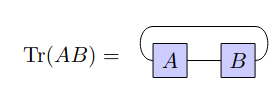
\includegraphics[width=0.4\textwidth]{trace}
		\centering
		\end{figure}
		
	\item Reduced density matrix (partial trace of bipartite state vector)
	\item SVD decomposition
		\begin{figure}[h]
		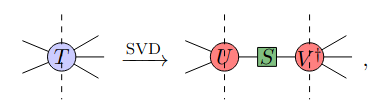
\includegraphics[width=0.6\textwidth]{svd}
		\centering
		\end{figure}
		\begin{itemize}
		\item Choice of index grouping, algorithm determine the bond dimension; independent of remaining discussion, set bond dimension as arbitrary value
		\end{itemize}
		
	\end{itemize}
\end{frame}

\begin{frame}{Matrix Product States}
	\begin{itemize}
		\item \textbf{MPS} : 1D array of tensors
		\begin{itemize}
		\item Two examples; open BC, periodic BC
		\item One tensor per site in many-body system; open indices represents physical degrees of freedom
		\item DoF : ${ pD^2N }$
		\end{itemize}
	\end{itemize}
	\begin{figure}[h]
	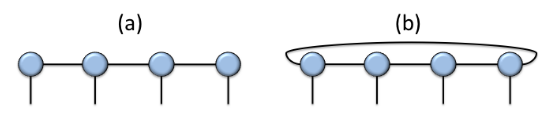
\includegraphics[width=0.8\textwidth]{mps}
	\centering
	\end{figure}
	
\end{frame}

\begin{frame}{Examples : MPS}
\begin{itemize}
	\item \textbf{GHZ State} : ${ \ket{\Psi }=\frac{1}{\sqrt{2}}(\ket{0}^{\otimes N}+\ket{1}^{\otimes N}) }$
		\begin{itemize}
		\item Maximally entangled state : reduced density matrix is diagonal for any bipartition of system
		\item MPS representation with bond dimension 2
		\end{itemize}
	\end{itemize}
	\begin{figure}[h]
	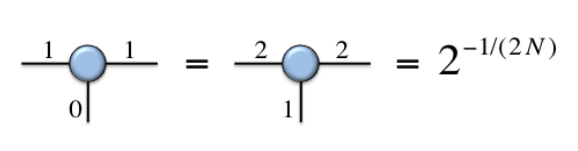
\includegraphics[width=0.6\textwidth]{ghz}
	\centering
	\end{figure}
	
\end{frame}

\begin{frame}{Examples : MPS}
	\begin{itemize}
		\item 1D PEPS (Projected Entangled Pair State)
			\begin{figure}[h]
			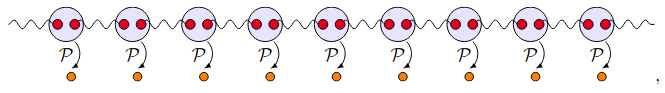
\includegraphics[width=0.8\textwidth]{peps1d}
			\centering
			\end{figure}
			
	\item Ground state of \textbf{1D AKLT} model : spin 1 chain with ${ H=\sum_{\ev{i,j}}^{} \boldsymbol{S}_{i}\cdot \boldsymbol{S}_{j}+ \frac{1}{3}(\boldsymbol{S}_{i}\cdot \boldsymbol{S}_{j})^{2} }$
		\begin{itemize}
		\item Exact ground state is given in terms of projection of a spin ${ \frac{1}{2} }$ chain
			\begin{figure}[h]
			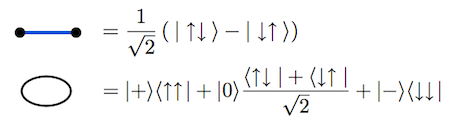
\includegraphics[width=0.5\textwidth]{aklt}
			\centering
			\end{figure}
			
		\item MPS representation with bond dimension 2
		\end{itemize}
	\end{itemize}
\end{frame}

\begin{frame}{Examples : MPS}
	\begin{itemize}
	\item \textbf{1D Cluster State} : simultaneous eigenket of ${ K^{i}=\sigma ^{x}_{i-1}\sigma ^{z}_{i}\sigma ^{x}_{i+1} }$; ${ \ket{\Psi }=\prod_i \frac{ 1+K^{i}}{2} \ket{0}^{\otimes N}}$
		\begin{itemize}
		\item Highly entangled state
		\item Represent operators ${ \frac{1+K^{i}}{2} }$ as TN
		\item MPS representation with bond dimension 4
		\end{itemize}
\end{itemize}	
\begin{figure}[h]
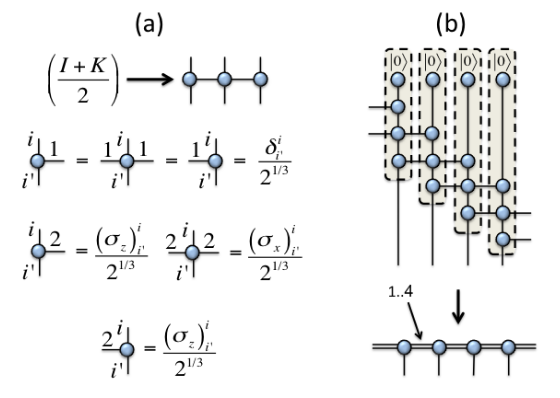
\includegraphics[width=0.5\textwidth]{1dcluster}
\centering
\end{figure}

\end{frame}


\begin{frame}{Physical Properties : MPS}
	\begin{itemize}
		\item MPS are dense
	\item Area law : constant entanglement entropy
		\begin{itemize}
		\item Split wavefunction into parts; ${ T_{\beta \gamma }=T^{\text{in}}_{\beta \alpha_1 \alpha_2} T^{\text{out}}_{\alpha _{1}\alpha _{2}\gamma }}$
			\begin{itemize}
			\item ${ \beta ,\gamma  }$ each indices of inner and outer state
			\item Combined indices ${ \overline{\alpha }=\{\alpha _{1},\alpha _{2}\} }$; total of ${ D^2  }$ values
			\item Roughly ${\ket{\psi }=\ket{\text{in}}\otimes \ket{\text{out}} }$
			\end{itemize}
		\item Reduced density matrix : ${ \rho_{\beta \beta ^{\prime}} ^{\text{in}}=T^{\text{out}}_{\overline{\alpha }\gamma }T^{\text{out}}_{\overline{\alpha }^{\prime}\gamma }T^{\text{in}}_{\beta \overline{\alpha }}T^{\text{in}}_{\beta^{\prime}\overline{\alpha }^{\prime}} }$
			\begin{itemize}
			\item Inner product between ${ T^{\text{out}} }$, outer product between ${ T^{\text{in}} }$
		\item wrt. ${ D }$, ${ \text{tr}\rho ^{\text{in}} }$ scales as ${ D^2  }$
		\item Const. wrt. subsystem size ${ L }$
		\item Roughly ${ \rho ^{\text{in}}=\ev{\text{out}|\text{out}}\ket{\text{in}}\bra{\text{in}} }$
			\end{itemize}
		\item ${ \alpha  }$-R\'enyi entropy : ${ S(L)= \frac{1}{1-\alpha }\log{\text{tr}\rho ^{\alpha }}\sim \log{D}}$
		\end{itemize}
	\end{itemize}
\end{frame}

\begin{frame}{Physical Properties : PEPS}
	\begin{figure}[h]
	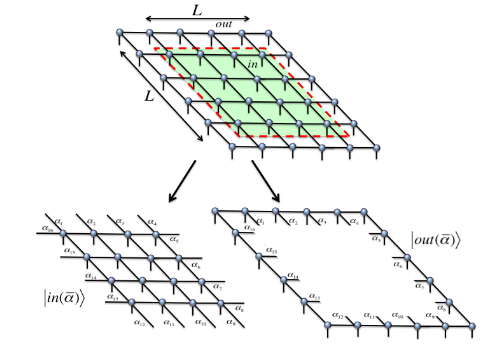
\includegraphics[width=0.8\textwidth]{peps}
	\centering
	\end{figure}
	\begin{itemize}
	\item ${ S(L)\sim 4L\log{D} }$
	\end{itemize}
\end{frame}


\begin{frame}{Physical Properties - Finitely Correlated : MPS}
\begin{itemize}
	\item Correlation function : ${ C(r)=\ev{O_{i}O^{\prime}_{i+r}} - \ev{O_{i}}\ev{O^{\prime}_{i+r}} }$\\
		Consider infinite MPS of single tensor; 1D translational invariance with thermodynamic limit
\end{itemize}	
	\begin{figure}[h]
	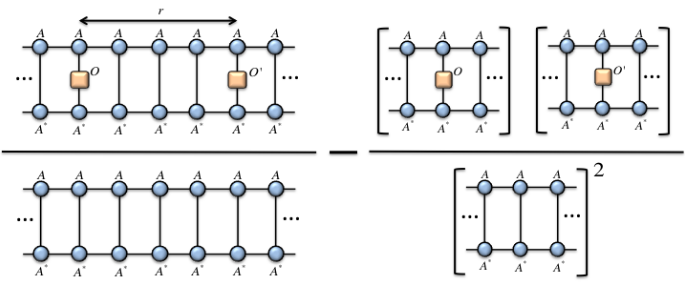
\includegraphics[width=0.8\textwidth]{corr}
	\centering
	\end{figure}
\end{frame}

\begin{frame}{Physical Properties - Finitely Correlated : MPS}
		\begin{figure}[h]
		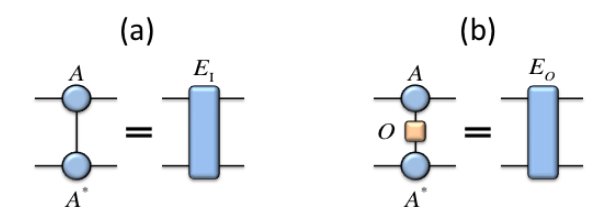
\includegraphics[width=0.6\textwidth]{fincor}
		\centering
		\end{figure}
	\begin{itemize}
		\item Consider ${ E_{i} }$ as ${ D^2 \times D^2  }$ matrix; diagonalise ${ E_{I} =\sum_{i=1}^{D^2 } \lambda _{i}\vec{R}_{i}^{T}\vec{L}_{i}}$; ${ E_{I}^{r}=\lambda _{1}^{r}\sum_{i=1}^{D^2 } (\lambda _{i}/\lambda _{1})^{r}\vec{R}_{i}^{T}\vec{L}_{i} }$
		\item Consider dominant EVs; ${ E_{I}^{r}\approx \lambda _{1}^{r}\left( \vec{R}_{1}^{T}\vec{L}_{1}+(\lambda _{2}/\lambda _{1})^{r} \sum_{}^{} \vec{R}_{\mu }^{T}\vec{L}_{\mu }\right)  }$
	\end{itemize}
\end{frame}

\begin{frame}{Physical Properties - Finitely Correlated : MPS}
	\begin{figure}[h]
	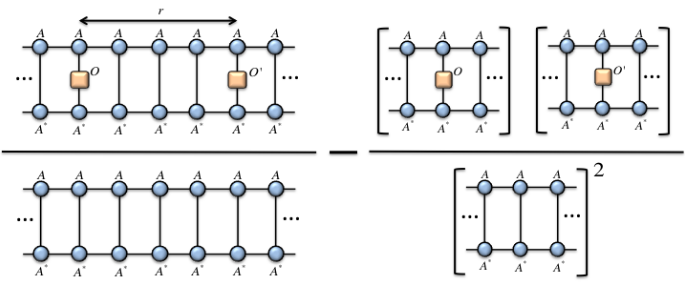
\includegraphics[width=0.8\textwidth]{corr}
	\centering
	\end{figure}
\begin{itemize}
\item ${ \ev{\psi |O_{i}|\psi }=\vec{L}_{1}E_{O}E_{I}^{r}\vec{R}_{1}^{T}}$\\
\item	In t.d. limit, ${ \ev{O_{i}}=\vec{L}_{1}E_{O}E_{I}^{r}\vec{R}_{1}^{T}/E_{I}^{r+1} =\vec{L}_{1}E_{O}\vec{R}_{1}^{T}/\lambda _{1}+\cdots }$
\item ${ \ev{O_{i}}\ev{O^{\prime}_{i+r}}\approx \vec{L}_{1}E_{O}\vec{R}_{1}^{T}\vec{L}_{1}E_{O^{\prime}} \vec{R}_{1}^{T}/\lambda _{1}^{2} }$

\end{itemize}
\end{frame}

\begin{frame}{Physical Properties - Finitely Correlated : MPS}
	\begin{figure}[h]
	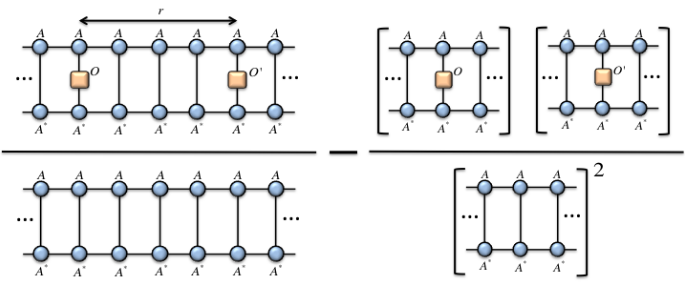
\includegraphics[width=0.8\textwidth]{corr}
	\centering
	\end{figure}
\begin{itemize}
\item ${ \ev{\psi |O_{i}O^{\prime}_{i+r}|\psi }=\vec{L}_{1}E_{O}E_{I}^{r-1}E_{O^{\prime}} \vec{R}_{1}^{T}}$\\
	\item	In t.d. limit, ${ \ev{O_{i}O^{\prime}_{i+r}}=\vec{L}_{1}E_{O}E_{I}^{r-1}E_{O^{\prime}}\vec{R}_{1}^{T}/E_{I}^{r+1}}$
	\item ${ \ev{O_{i}O_{i+r}^{\prime}}=\vec{L}_{1}E_{O}\vec{R}_{1}^{T}\vec{L}_{1}E_{O^{\prime}}\vec{R}_{1}^{T}/\lambda _{1}^{2} +(\lambda _{2}/\lambda _{1})^{r}\sum_{}^{} \vec{R}^{T}_{\mu} \vec{L}_{\mu }}$
	\item ${ C(r)\sim \exp -r/\xi }$ with ${ \xi =-1  /\log{|\lambda _{1}/\lambda _{2}|}}$

\end{itemize}
\end{frame}

\begin{frame}{Physical Properties - Finitely Correlated : MPS}
	\begin{itemize}
	\item Exponential decay of two-point correlation function
	\item Results known where such exponential decay \textit{implies} the area law
	\item Correlation function mimics quantum system in lower spatial dimension
	\end{itemize}
\end{frame}

\begin{frame}{MPS Algorithms}
% choice of bond dimension?
		How do we use TNs in calculations? What are the considerations we must make?
		\vspace{.5cm}
	\begin{itemize}
	\item Approximation of general tensors into TN states
	\item Calculating ground states
		\begin{itemize}
		\item Variational method over TN space; DMRG, TEBD
		\item Imaginary time evolution
		\end{itemize}
	\item (Efficient) computation of expectation values of TN states
	\end{itemize}
\end{frame}



\begin{frame}{MPS Algorithms}
	\begin{itemize}
	\item Can we decompose an arbitrary rank N tensor into an MPS state? Yes! By recursively applying SVD
		\begin{itemize}
		\item For ${ N }$ particle system, bond dimension is bounded above by ${ 2^{\lfloor N/2\rfloor}}$; MPS are dense
		\item Expensive in terms of calculations
		\end{itemize}
	\end{itemize}
\end{frame}

\begin{frame}{MPS Algorithms}
	\begin{itemize}
				\item \textbf{Rank} : distinct from rank of tensor, dimensionality of image
					\begin{itemize}
			\item Ex. ${ m \times n }$ matrix of rank one : outer product of ${ m }$ vector and ${ n }$ vector
			\item ${ m \times  n }$ matrix of rank ${ k }$ : total ${ k(m+n) }$ DoF
			\item Imposing low rank conditions on TNs further compresses the data
				\end{itemize}
		\item \textbf{Low rank approximation}
			\begin{itemize}
				\item Eckart-Young theorem : optimal low rank approximation appears via SVD
				\item Truncate to ${ k }$ singular values
			\end{itemize}
		\item Use low rank approximation to apply cutoff to bond dimension of MPS; approximation of general state
		%\item Can also heuristically choose to cutoff of singular values at $\xi ={ \frac{1}{\sqrt{p^{N}}} }$; error is ${ \mathcal{O}(\xi^2) }$
	\end{itemize}
	
\end{frame}


\begin{frame}{MPS Algorithms}
	\begin{itemize}
	\item Iteratively improve approximations by using variational methods; ex. \textbf{Density Matrix Renormalisation Group}
	\item Time evolve MPSs via nearest-neighbour Hamiltonians; ex. \textbf{Time-Evolving Block Decimation}
	\end{itemize}
\end{frame}

%\begin{frame}{MPS Algorithms : DMRG}
%	\begin{itemize}
%	\item 
%	\end{itemize}
%\end{frame}

%\begin{frame}{MPS Algorithms : TEBD}
%	\begin{itemize}
%	\item 
%	\end{itemize}
%\end{frame}

%\begin{frame}{TN Algorithms : MPS EV}
%	\begin{figure}[h]
%	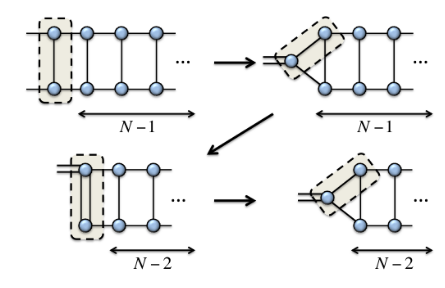
\includegraphics[width=0.75\textwidth]{mpscontr}
%	\centering
%	\end{figure}
%	
%\end{frame}

%\begin{frame}{TN Algorithms : PEPS EV}
%	\begin{itemize}
%	\item Contraction of a 2D lattice is computationally complex
%	\item Approximation required; reduce the original problem to a series of 1D problems equivalent to the ground state calculations problems above!\\
%		Return to this problem later
%\end{itemize}
%\end{frame}

\begin{frame}{References and Resources}
	\begin{itemize}
	\item Hand-waving and Interpretive Dance : An Introductory Course on Tensor Networks; Jacob C. Bridgeman, Christopher T. Chubb
	\item A Practical Introduction to Tensor Networks : Matrix Product States and Projected Entangled Pair States; Rom\'an Or\'us
	\item The density-matrix renormalization group in the age of matrix product states; Ulrich Schollw\"ock
	\end{itemize}
\end{frame}

\end{document}

